\documentclass{article}

\usepackage{graphicx} % Required for inserting images

\usepackage{darkmode}
\usepackage{tikz}

\usepackage{geometry}

\usepackage{amsmath}

\usetikzlibrary{calc}
% \newcommand*{\rom}[1]{\expandafter\@slowromancap\romannumeral #1@}

\sloppy
% \enabledarkmode

\colorlet{boxfillcolor}{gray!10}

\title{Calc II notes}
\author{Pierson Lipschultz}
\date{March 2025}

\begin{document}



\vspace*{\fill}
\begingroup
\begin{center}
    \huge
    Calc II Notes

    Pierson L
    
\end{center}

\endgroup
\vspace*{\fill}

\newgeometry{left=0.25in, right=0.25in, top=0.5in, bottom=0.5in}
\vspace*{\fill}
\begingroup
\noindent
    \resizebox{\dimexpr\paperwidth-5em}{!}{%
        \centering
        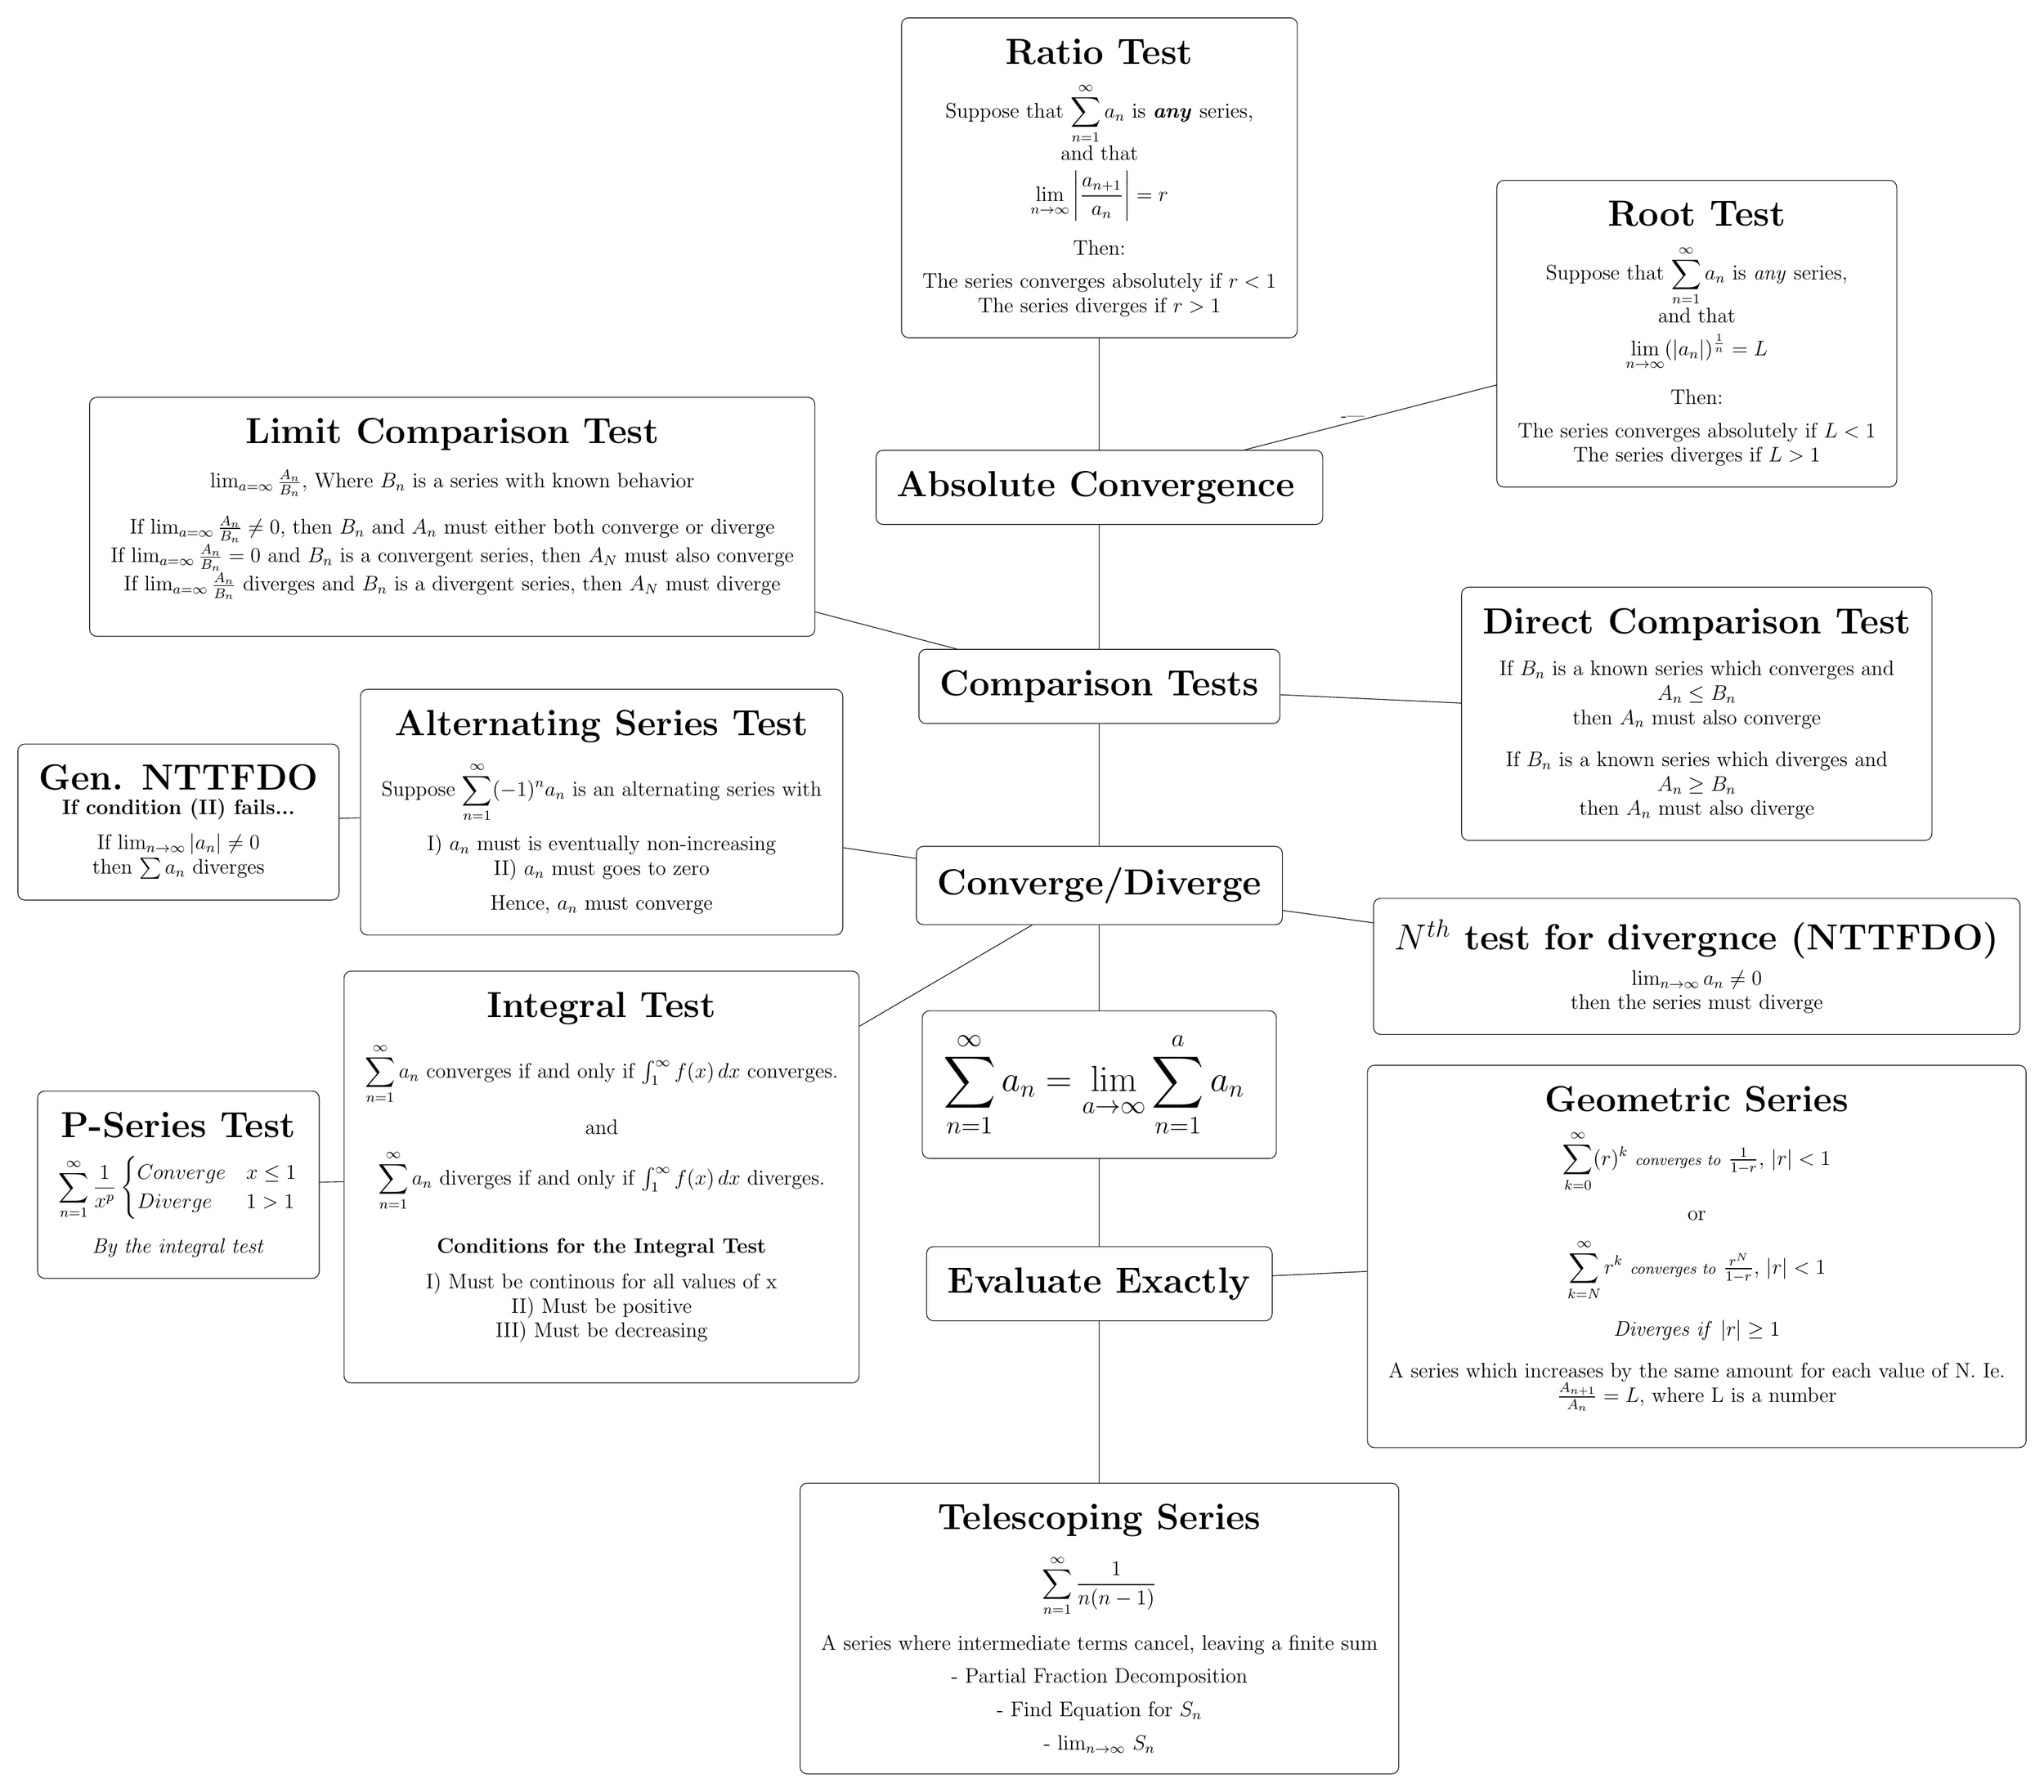
\begin{tikzpicture}

            \tikzstyle{box} = [shape=rectangle, draw=black, align=center, rounded corners, inner sep=12pt, font =\large] 

            %titles and jazz

            %main
            \node[box] (Main) at (0,0) {
                \huge $\displaystyle \sum_{n=1}^{\infty} a_n = \lim_{a \rightarrow \infty}\sum_{n=1}^{a} a_n$
            };

            %evalulate 
            \node[box](EvalExc) at (0,-4) {\huge \textbf{Evaluate Exactly}};

            %Converge or Diverge
            \node[box] (CorD) at (0,4){\huge \textbf{Converge/Diverge}};
            
            %NTTFDO
            \node[box, anchor=south] (NTTFDO) at (12,1){\huge \textbf{$N^{th}$ test for divergnce (NTTFDO)} \\ [6pt] 
            $\lim_{n \rightarrow \infty} a_n \neq 0$ \\
            then the series must diverge
            };
            
            %Comp tests
            \node[box] (CompT) at (0,8){\huge \textbf{Comparison Tests}};

            %Absolute convergence 
            \node[box] (ABSConvg) at (0,12){
                {\huge \textbf{Absolute Convergence}}
                };
                            
            %limit comp text
            \node[box, anchor=south] (LCT) at (-13,9){
                {\huge \textbf{Limit Comparison Test}} \\[10pt]
                $\lim_{ a = \infty} \frac{A_n}{B_n}$, Where $B_n$ is a series with known behavior\\ [10pt]
                If $\lim_{ a = \infty} \frac{A_n}{B_n}\neq 0$, then $B_n$ and $A_n$ must either both converge or diverge\\
                If $\lim_{ a = \infty} \frac{A_n}{B_n} = 0$ and $B_n$ is a convergent series, then $A_N$ must also converge\\
                If $\lim_{ a = \infty} \frac{A_n}{B_n}$ diverges and $B_n$ is a divergent series, then $A_N$ must diverge\\

            };

            %direct comp text
            \node[box, anchor=north] (DCT) at (12,10){
                {\huge \textbf{Direct Comparison Test}}\\[10pt]
                If $B_n$ is a known series which converges and\\
                $A_n \leq B_n$\\
                then $A_n$ must also converge\\[10pt]

                If $B_n$ is a known series which diverges and\\
                $A_n \geq B_n$\\
                then $A_n$ must also diverge
            };

            %Ratio Test
            \node[box, anchor=south] (RatioTest) at (0,15){
                {\huge \textbf{Ratio Test}}\\[10pt]
                Suppose that $\displaystyle \sum_{n=1}^{\infty} a_n$ is \textit{\textbf{any}} series,\\
                and that\\[5pt]
                $\displaystyle \lim_{n \rightarrow \infty} \left| \frac{a_{n+1}}{a_n} \right| = r$\\[10pt]
                Then: \\[5pt]
                The series converges absolutely if $r < 1$\\
                The series diverges if $r > 1$
                };

            %Root Test
            \node[box, anchor=south] (RootTest) at (12,12){
                {\huge \textbf{Root Test}}\\[10pt]
                Suppose that $\displaystyle \sum_{n=1}^{\infty} a_n$ is \textit{any} series,\\
                and that\\[5pt]
                $\displaystyle \lim_{n \rightarrow \infty} ({|a_n|})^\frac{1}{n} = L$\\[10pt]
                Then: \\[5pt]
                The series converges absolutely if $L < 1$\\
                The series diverges if $L > 1$
                };

            %Telescoping
            \node[box, anchor=north] (Tele) at ($(EvalExc)+(0,-4)$) {
                \textbf{\huge Telescoping Series} \\[10pt]
                $\displaystyle \sum_{n=1}^{\infty} \frac{1}{n(n-1)}$ \\[10pt]
                A series where intermediate terms cancel, leaving a finite sum \\[5pt]
                - Partial Fraction Decomposition  \\[5pt]
                - Find Equation for $S_n$ \\[5pt]
                - $\lim_{n \to \infty}$ $S_n$
            };

            %Geometric
            \node[box, anchor=south] (Geom) at (12,-7.3) {
                \textbf{\huge Geometric Series} \\[10pt]
                $\displaystyle \sum_{k=0}^{\infty} (r)^k$ \textit{\small converges to} $\frac{1}{1-r},$ $|r| < 1 $ \\[10pt] 
                or \\[10pt]
                $\displaystyle \sum_{k=N}^{\infty} r^k$ \textit{\small converges to} $\frac{r^N}{1-r}, $ $|r| < 1 $\\[10pt]
                \textit{Diverges if} $\left|r\right| \geq 1$\\ [10pt]
                A series which increases by the same amount for each value of N. Ie. \\
                $\frac{A_{n+1}}{A_n} = L$, where L is a number \\ 
                
            };

            %Integral Test
            \node[box, anchor=south] (IntTest) at (-10,-6){\huge \textbf{Integral Test} \\ [10pt]
            $\displaystyle \sum_{n=1}^{\infty} a_n$ converges if and only if $\int_1^\infty f(x) \, dx$ converges. \\ [8pt]
            and \\ [8pt]
            $\displaystyle \sum_{n=1}^{\infty} a_n$ diverges if and only if $\int_1^\infty f(x) \, dx$ diverges. \\ [15pt]

            \textbf{Conditions for the Integral Test} \\ [6pt]
            I) Must be continous for all values of x\\
            II) Must be positive\\
            III) Must be decreasing \\ 

            
            };

            %Alternating Series Test
            \node[box, anchor=south] (AltSerTest) at (-10,3){\huge \textbf{Alternating Series Test} \\ [10pt]
            Suppose $\displaystyle \sum_{n=1}^{\infty} (-1)^n a_n$ is an alternating series with\\ [6pt]
            I) $a_n$ must is eventually non-increasing\\
            II) $a_n$ must goes to zero\\ [6pt]
            Hence, $a_n$ must converge

            };

            %Generalized NTTFDO

            \node[box, anchor=south] (GenNTTFDOTest) at (-18.5,3.7){
            \huge \textbf{Gen. NTTFDO}\\ 
            \textbf{If condition (II) fails...}\\ [6pt]
            If $\lim_{n \rightarrow \infty} \left|a_n \right| \neq 0$ \\
            then $\sum a_n$ diverges 
            };

            %p-series test
            \node[box, anchor=south] (PSes) at (-18.5,-3.9){\huge \textbf{P-Series Test}\\ [10pt]
            
            $\displaystyle \sum_{n=1}^{\infty} \frac{1}{x^p} \begin{cases} 
            Converge & x\leq 1 \\
            Diverge & 1 > 1 \\ 
            \end{cases}$ \\ [10pt]
            
            \textit{By the integral test} 
            
            };



            \path [-] (Main) edge node[left] {$$} (EvalExc);
            \path [-] (EvalExc) edge node[left] {$$} (Tele);
            \path [-] (EvalExc) edge node[left] {$$} (Geom);
            \path [-] (Main) edge node[left] {$$} (CorD);
            \path [-] (CorD) edge node[left] {$$} (NTTFDO);
            \path [-] (CorD) edge node[left] {$$} (IntTest);
                \path [-] (IntTest) edge node[left] {$$} (PSes);
            \path [-] (CorD) edge node[left] {$$} (CompT);
                \path [-] (CompT) edge node[left] {$$} (LCT);
                \path [-] (CompT) edge node[left] {$$} (DCT);
                \path [-] (CompT) edge node[left] {$$} (ABSConvg);
                    \path [-] (ABSConvg) edge node[left] {$$} (RatioTest); 
                    \path [-] (ABSConvg) edge node[left] {-|} (RootTest); 
            \path [-] (CorD) edge node[left] {$$} (AltSerTest);
                \path [-] (AltSerTest) edge node[left] {$$} (GenNTTFDOTest);




        \end{tikzpicture}
    }

\endgroup
\vspace*{\fill}
\restoregeometry
\pagebreak

\section{\centering \huge Absolute Convergence \\ \fbox{10.5}}
    \subsection{Good Practice Problems}
        \fbox{\textit{57}}
    \subsection{Ratio Test} 
    \hrulefill \\[10pt]

    The Ratio Test\footnote{Very important regarding factorials} states that 
        
        \begingroup
        \centering
        Suppose that $\displaystyle \sum_{n=1}^{\infty} a_n$ is \textit{\textbf{any}} series,\\
        and that\\[5pt]\textbf{}
        $\displaystyle \lim_{n \rightarrow \infty} \left| \frac{a_{n+1}}{a_n} \right| = r$\\[10pt]
        Then: \\[5pt]
        The series converges absolutely if $r < 1$\\
        The series diverges if $r > 1$\\
        \endgroup
    \subsubsection{"Keys"}
        \hrulefill\\ [5pt]
        \begingroup
        \centering
        \large
        
        $\displaystyle \frac{a^{n+1}}{a^n} = a$, ~~~~ $\displaystyle \frac{a^{n}}{a^{n+1}} = \frac{1}{a}$ \\ [15pt]



        $\displaystyle \frac{(n+1)^{a}}{n^{a}} = \left(1+\frac{1}{n}\right)^a$ \\ [15pt]

        $\displaystyle \frac{(n+1)!}{n!} = (n + 1) $\\ [15pt]

        \textit{Note that these can be combined} \\ [5pt]
        \fbox{Example}
        $\frac{2^{n+1}(n+1)!}{2^n(n!)} = 2(n+1)$



        \endgroup
    \subsubsection{Examples}    

        \begingroup
        \centering

        \fbox{\large \textbf{Example 1}}\\

        \hrulefill \\[10pt]

        \fbox{\large Simplify $\frac{(n+2)!}{(n-1)!}$}\\[5pt]
        \textit{Ratio of factorials}\\[15pt]

        $=\frac{(n+2)!}{(n-1)!}$\\[15pt]
        
        $= \frac{(n+1)(n+1)(n)(n-1)\cdots(1)}{(n-1)(n-2)(n-3)\cdots(1)}$\\[15pt]
        
        $= \frac{(n+1)(n+1)(n)(n-1)}{(n-1)}$\\[15pt]

        $= {(n+1)(n+1)(n)}$\\[15pt]
\pagebreak
        \endgroup

        \begingroup 
        \centering
        \fbox{\large \textbf{example 2}}\\
        \hrulefill \\[10pt]

        \textit{Problem 57 from book}\\ [15pt]
        
        \fbox{$\displaystyle \sum_{n=1}^{\infty} \frac{2^n(n!)^2}{2n!}$} \\ [10pt]
        We apply the Ratio test \\ [15pt]

        $\displaystyle \lim_{n \rightarrow \infty} \frac{\frac{(2^{n+1})(n+1)!^2}{2(n+1)!}}{\frac{2^nn!^2}{2n!}}$\\ [10pt]

        $\displaystyle \lim_{n \rightarrow \infty} \frac{2^{n+1}(n+1)^2}{2(n+1)} \times \frac{2n!}{2n(n!)^2}$\\[10pt]

        $\displaystyle \lim_{n \rightarrow \infty} \frac{2^{n+1}(n+1)^2}{\textbf{2n+2}}\times \frac{2n!}{2n(n!)^2}$,      {\tiny note the +2}\\[10pt]

        $\displaystyle \lim_{n \rightarrow \infty} \frac{2(n+1)^2}{\textbf{(2n+2)(2n+1)}}$ \\ [10pt]
        $= \frac{1}{2} < 1$\\ [15pt]
        Hence, the series $\displaystyle \sum_{n=1}^{\infty} \frac{2^n(n!)^2}{2n!}$ converges\\

        \endgroup
    \pagebreak


    \section{Alternating Series}
    \hrulefill\\ [15pt]
    \begingroup 
    \centering

    Suppose $\displaystyle \sum_{n=1}^{\infty} (-1)^n a_n$ is an alternating series with\\ [6pt]
                I) $a_n$ eventually non-increasing\\
                II) $a_n$ going to zero\\ [6pt]
                Then, $a_n$ must converge\\ [80pt]
    \endgroup
    
    \begingroup
    \centering
    
    \begingroup
    \centering
        \large
        \fbox{$\sum_{n=1}^{\infty}\frac{1}{n}$}
    \endgroup

    \resizebox{\dimexpr\textwidth-5em}{!}{%
    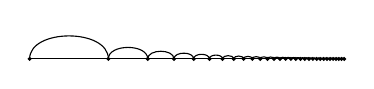
\begin{tikzpicture}

    \draw[thin] (0, 0) -- (3.995, 0);

    \foreach \i in {0, 1.0, 1.5, 1.8333, 2.0833, 2.2833, 2.45, 2.5929, 2.7179, 2.829, 2.929, 3.0199, 3.1032, 3.1801, 3.2516, 3.3182, 3.3807, 3.4396, 3.4951, 3.5477, 3.5977, 3.6454, 3.6908, 3.7343, 3.776, 3.816, 3.8544, 3.8915, 3.9272, 3.9617, 3.995}
        \node[draw, circle, inner sep=.1pt, fill=black] at (\i, 0) {};
 
    \foreach \A/\B in {0/1, 1.0/1.5, 1.5/1.8333, 1.8333/2.0833, 2.0833/2.2833, 2.2833/2.45, 2.45/2.5929, 2.5929/2.7179, 2.7179/2.829, 2.829/2.929, 2.929/3.0199, 3.0199/3.1032, 3.1032/3.1801, 3.1801/3.2516, 3.2516/3.3182, 3.3182/3.3807, 3.3807/3.4396, 3.4396/3.4951, 3.4951/3.5477, 3.5477/3.5977, 3.5977/3.6454, 3.6454/3.6908, 3.6908/3.7343, 3.7343/3.776, 3.776/3.816, 3.816/3.8544, 3.8544/3.8915, 3.8915/3.9272, 3.9272/3.9617, 3.9617/3.995}
        \draw (\A, 0) to[bend left=90] (\B, 0);
        
    \end{tikzpicture}
    } \\ [40pt]

    \begingroup
    \centering
        \large
        \fbox{$\sum_{n=1}^{\infty}\frac{(-1)^n}{n}$}
    \endgroup

    \resizebox{\dimexpr\textwidth-5em}{!}{%
    \begingroup 
    \centering
    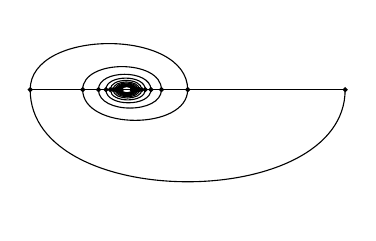
\begin{tikzpicture}

    \draw[thin] (0, 0) -- (-4, 0);

    \foreach \i in {0, -1.0, -0.5, -0.8333, -0.5833, -0.7833, -0.6167, -0.7595, -0.6345, -0.7456, -0.6456, -0.7365, -0.6532, -0.7301, -0.6587, -0.7254, -0.6629, -0.7217, -0.6661, -0.7188, -0.6688, -0.7164, -0.6709, -0.7144, -0.6727, -0.7127, -0.6743, -0.7113, -0.6756, -0.7101, -0.6768}
        \node[draw, circle, inner sep=.5pt, fill=black] at (\i*4, 0) {};
    
    

    \foreach \A/\B in {0/-1.0, -1.0/-0.5, -0.5/-0.8333, -0.8333/-0.5833, -0.5833/-0.7833, -0.7833/-0.6167, -0.6167/-0.7595, -0.7595/-0.6345, -0.6345/-0.7456, -0.7456/-0.6456, -0.6456/-0.7365, -0.7365/-0.6532, -0.6532/-0.7301, -0.7301/-0.6587, -0.6587/-0.7254, -0.7254/-0.6629, -0.6629/-0.7217, -0.7217/-0.6661, -0.6661/-0.7188, -0.7188/-0.6688, -0.6688/-0.7164, -0.7164/-0.6709, -0.6709/-0.7144, -0.7144/-0.6727, -0.6727/-0.7127, -0.7127/-0.6743, -0.6743/-0.7113, -0.7113/-0.6756, -0.6756/-0.7101, -0.7101/-0.6768}
    \draw[thin] (\A*4, 0) to[bend left=90] (\B*4, 0);


    \end{tikzpicture}
    \endgroup
    }
    

    \subsection{Examples}
        \centering
        \hrulefill \\ [15pt]
        \fbox{Example 1}
        $\displaystyle \sum_{n=1}^{\infty} \frac{(-1)^n}{n}$, Converge or diverge? \\ [15pt]

        We apply the Alternating Series Test (AST) \\ [15pt]

        $a_n = \frac{1}{n}$\\ [10pt]

        1) $\frac{1}{n+1} < \frac{1}{n} \rightarrow Decreasing$\\ [8pt]
        2) $\displaystyle \lim_{n \rightarrow \infty} a_n = \lim_{n \rightarrow \infty} \frac{1}{n} = 0$\\ [20pt]
        Hence, by AST, the series converges \textbf{conditionally}

\pagebreak
\section{\centering \huge Misc}
    \centering
    \subsection{\huge Factorials}
    \fbox{\large ex.1}

        \hrulefill \\[10pt]

            \fbox{\large 4! = 4 x 3! = 4x3x2! = 4x3x2x1! = 4x3x2x1x0!}

            $\rightarrow$

            \fbox{0! = 1}

            $\rightarrow$

            \fbox{4!= 24}

            \hrulefill \\[10pt]

    \fbox{\large \textbf{ex. 2}}\\

    \hrulefill \\[10pt]

    \fbox{\large Simplify $\frac{(n+2)!}{(n-1)!}$}\\[5pt]
    \textit{Ratio of factorials}\\[15pt]

    $=\frac{(n+2)!}{(n-1)!}$\\[15pt]
    
    $= \frac{(n+1)(n+1)(n)(n-1)\cdots(1)}{(n-1)(n-2)(n-3)\cdots(1)}$\\[15pt]
    
    $= \frac{(n+1)(n+1)(n)(n-1)}{(n-1)}$\\[15pt]

    $= {(n+1)(n+1)(n)}$\\[15pt]


\end{document}
